\documentclass[a4paper,UTF8]{article}
\usepackage{ctex}
\usepackage[margin=1.25in]{geometry}
\usepackage{color}
\usepackage{graphicx}
\usepackage{amssymb}
\usepackage{amsmath}
\usepackage{amsthm}
\usepackage{enumerate}
\usepackage{bm}
\usepackage{hyperref}
\usepackage{epsfig}
\usepackage{color}
\usepackage{tcolorbox}
\usepackage{mdframed}
\usepackage{lipsum}
\usepackage{subfigure}
\newmdtheoremenv{thm-box}{myThm}
\newmdtheoremenv{prop-box}{Proposition}
\newmdtheoremenv{def-box}{定义}

\setlength{\evensidemargin}{.25in}
\setlength{\textwidth}{6in}
\setlength{\topmargin}{-0.5in}
\setlength{\topmargin}{-0.5in}
% \setlength{\textheight}{9.5in}
%%%%%%%%%%%%%%%%%%此处用于设置页眉页脚%%%%%%%%%%%%%%%%%%
\usepackage{fancyhdr}                                
\usepackage{lastpage}                                           
\usepackage{layout}                                             
\footskip = 10pt 
\pagestyle{fancy}                    % 设置页眉                                                                                                                                                              
\cfoot{\thepage}                                                
\renewcommand{\headrulewidth}{1pt}  			%页眉线宽,设为0可以去页眉线
\setlength{\skip\footins}{0.5cm}    			%脚注与正文的距离           
\renewcommand{\footrulewidth}{0pt}  			%页脚线宽,设为0可以去页脚线

\makeatletter 									%设置双线页眉                                        
\def\headrule{{\if@fancyplain\let\headrulewidth\plainheadrulewidth\fi%
\hrule\@height 1.0pt \@width\headwidth\vskip1pt	%上面线为1pt粗  
\hrule\@height 0.5pt\@width\headwidth  			%下面0.5pt粗            
\vskip-2\headrulewidth\vskip-1pt}      			%两条线的距离1pt        
\vspace{6mm}}     								%双线与下面正文之间的垂直间距              
\makeatother  

%%%%%%%%%%%%%%%%%%%%%%%%%%%%%%%%%%%%%%%%%%%%%%
\numberwithin{equation}{section}
%\usepackage[thmmarks, amsmath, thref]{ntheorem}
\newtheorem{myThm}{myThm}
\newtheorem*{myDef}{Definition}
\newtheorem*{mySol}{Solution}
\newtheorem*{myProof}{Proof}
\newcommand{\indep}{\rotatebox[origin=c]{90}{$\models$}}
\newcommand*\diff{\mathop{}\!\mathrm{d}}

\usepackage{multirow}

% 子标题
\usepackage{titling}
\newcommand{\subtitle}[1]{%
	\posttitle{%
		\par\end{center}
	\begin{center}\large#1\end{center}
	\vskip0.5em}%
}

%算法包
\usepackage{caption}
\usepackage{algorithm,float}
\usepackage{algorithmic}
%算法input output
\renewcommand{\algorithmicrequire}{\textbf{Input:}} % Use Input in the format of Algorithm
\renewcommand{\algorithmicensure}{\textbf{Output:}} % Use Output in the format of Algorithm
\DeclareMathOperator*{\argminA}{arg\,min} % Jan Hlavacek

%代码包
\usepackage{listings}
\usepackage{color}
\usepackage{xcolor}
\definecolor{dkgreen}{rgb}{0,0.6,0}
\definecolor{gray}{rgb}{0.5,0.5,0.5}
\definecolor{mauve}{rgb}{0.58,0,0.82}
\lstset{frame=tb,
	language=Java,
	aboveskip=3mm,
	belowskip=3mm,
	showstringspaces=false,
	columns=flexible,
	basicstyle = \ttfamily\small,
	numbers=none,
	numberstyle=\tiny\color{gray},
	keywordstyle=\color{blue},
	commentstyle=\color{dkgreen},
	stringstyle=\color{mauve},
	breaklines=true,
	breakatwhitespace=true,
	tabsize=3
}

\begin{document}
\title{MapReduce 课程设计:金庸的江湖}
\subtitle{   \ \ \ \ ——分析小说中人物关系}
\author{朱庭纬,崔子寒,吴昌容}
\maketitle
\tableofcontents
\newpage
\begin{abstract}
	这是中文摘要
\end{abstract}
\newcommand{\enabstractname}{Abstract}
\newenvironment{enabstract}{%
	\par\small
	\noindent\mbox{}\hfill{\bfseries \enabstractname}\hfill\mbox{}\par
	\vskip 2.5ex}{\par\vskip 2.5ex} 
\begin{enabstract}
	this is abstract
\end{enabstract}
\newpage
\section{实验要求}
\subsection{数据预处理:分词}
从原始的小说文本中,抽取与人物互动相关的数据,屏蔽掉与人物关系无关的文本内容,为后面基于人物共现的分析做准备。\\
\textbf{输入}:1. 金庸全本武侠小说文集(未分词);2. 金庸武侠小说人名列表。\\
\textbf{输出}:分词后,仅保留人名的武侠小说全集。
\subsection{特征提取:单词同现}
在人物同现分析中,如果两个人在原文的同一段落中出现,则认为两个人发生了一次同现关系。需要对人物之间的同现关系次数进行统计,同现关系次数越多,则说明两人关系越密切。\\
\textbf{输入}:分词后仅保留人名的武侠小说全集。\\
\textbf{输出}:在金庸的所有武侠小说中,人物之间的同现次数。
\subsection{归一化}
获得人物之间的同现次数后,根据同现关系生成人物之间的关系图。在关系图中,人物是顶点,人物之间的互动关系是边。边的权值是两个人之间的共现概率。\\
\textbf{输入}:人物共现次数矩阵。\\
\textbf{输出}:权重归一化后的人物关系图。
\subsection{PageRank}
获得权重归一化化后的人物关系图后,可以进行数据分析任务。PageRank是典型的数据分析任务,通过PageRank可以确定金庸武侠江湖中的“主角”是哪些。\\
\textbf{输入}:权重归一化后的人物关系图。
\\\textbf{输出}:人物的PageRank值。
\subsection{标签传播}
标签传播(Label Propagation)是一种半监督的图分析算法,它能为图上的顶点打上标签,进行图顶点的聚类分析。通过在人物关系图上进行标签传播,可以将属于同一本书的人物聚为一类。\\
\textbf{输入}:权重归一化后的人物关系图。\\
\textbf{输出}:人物的标签信息。
\subsection{输出整理}
对于PageRank的结果,可以使用MapReduce任务按照PageRank值进行全局排序。\\
对于标签传播的结果,可以使用MapReduce任务将属于同一标签的任务输出到一起,便于结果查看。
\section{小组分工}
\begin{table}[!htbp]
	\centering
	\caption{小组分工}
	\begin{tabular} {|p{50pt}|p{80pt}|p{260pt}|}
		\hline
		姓名& 学号 &任务\\
		\hline
		朱庭纬&161220186&数据预处理,特征提取归一化,数据可视化,报告撰写\\
		\hline
		崔子寒&161220026&PageRank,结果整理,数据可视化,报告撰写\\
		\hline
		吴昌容&161220134&标签传播任务,结果整理,报告撰写\\
		\hline
	\end{tabular}
\end{table}
\section{实验环境}
\begin{table}[!htbp]
	\centering
	\caption{实验环境}
	\begin{tabular} {|p{80pt}|p{160pt}|}
		\hline
		操作系统&Ubuntu 18.04 LTS\\
		\hline
		hadoop版本& 2.7.1\\
		\hline
		jdk版本& 1.7.0\\
		\hline
		构建工具&Maven\\
		\hline
	\end{tabular}
\end{table}
\section{编译、打包、运行}
\subsection{编译打包}
由于使用Maven作为构建工具,所以可以很方便的添加依赖,我们在pom.xml文件中添加了表3所示的依赖:
\begin{table}[!htbp]
	\centering
	\caption{项目依赖}
	\begin{tabular} {|p{90pt}|p{250pt}|p{50pt}|}
		\hline
		groupId& artifactId &version\\
		\hline
		org.apache.hadoop&hadoop-mapreduce-client-core&2.6.0\\
		\hline
		org.apache.hadoop&hadoop-test&1.2.1\\
		\hline
		org.apache.hadoop&hadoop-common&2.7.1\\
		\hline
		org.ansj&ansj\_seg&5.1.6\\
		\hline
	\end{tabular}
\end{table}
\\
其中,groupId为org.apache.hadoop的三个依赖是hadoop MapReduce API的有关依赖。ansj\_seg是分词库的依赖,这里使用的是官网上最新的5.1.6版本。\\
为了在打包时将第三方的依赖和代码一起打包,使用Maven插件org.apache.maven.plugins: maven-shade-plugin,通过设置目标为shade,可以将依赖连同代码一起打包。打包的命令为:\textbf{mvn package -Dhttps.protocols=TLSv1.2}。 由于我们使用的jdk版本是1.7,而1.7默认的https协议是TLSv1.1,现在maven仓库已经不再支持这个版本的协议,所以需要加上参数,否则在下载依赖时会出错。
\subsection{运行方式}
任务代码由三名成员合作编写,每人负责一个模块,然后将模块组合起来。运行时既可以通过运行主类Main,依次运行所有任务,也可以分别运行某一个子任务。具体的运行方式如表4所示(假设jar包名称为jianghu.jar):
\begin{table}[!htbp]
	\centering
	\caption{运行方式}
	\begin{tabular} {|p{180pt}|p{300pt}|}
		\hline
		指令&解释\\
		\hline
		hadoop jar jianghu.jar cn.nju.st13.Main arg0 arg1 arg2&arg0:小说文件夹路径;arg1:人名文件路径;arg2:输出结果路径\\
		\hline
		hadoop jar  jianghu.jar  cn.nju.st13.preprocess.Preprocess arg0 arg1 arg2 arg3&arg0:小说文件夹路径;arg1:人名文件路径;arg2:人物关系图输出路径;arg3:可选参数"-1","-2","-3",代表三种不同的方法\\
		\hline
		hadoop jar jianghu.jar cn.nju.st13.pagerank.PageRankDriver arg0 arg1 可选参数&arg0:人物关系图路径;arg1:排序处理后的PageRank结果路径;可选参数:-max\_iter=n(n为最大迭代次数,默认15),-retain\_process=false/true(是否保留中间结果,默认false)\\
		\hline
		hadoop jar jianghu.jar cn.nju.st13.labelprop.LabelProp arg0 arg1&arg0:人物关系图路径;arg1:整理后的标签传播算法结果路径。\\
		\hline
	\end{tabular}
\end{table}

\section{算法介绍}
\subsection{数据预处理}
首先我们需要从原始文本中把文章中所有的人名抽取出来,屏蔽掉其他与人物关系分析任务无关的内容。要完成此任务有两个步骤:将段落分割成词语,再从所有词语中过滤出金庸小说中的人物名字。\\
\indent 问题的关键在于如何正确分词,使得目标人名能够被正确提取。我们使用的分词工具是Ansj\_seg,在分词前向词典中添加所有自定义词语即可。分词后判断每个词语的词性是否为“nr”(即人名)以及是否在给定的人名列表中即可提取出所有人物名称。\\
\indent 由于每行的处理方式均相同,仍可采用mapreduce进行并行处理。在mapper端代码中,在setup函数中读取人名列表,将列表中每个人名添加到词典中;在map函数中,对于每一行,将分词结果存入Result类型变量中,然后根据词性和是否在人名列表中判断每个词是否为目标人名。最后将所有目标人名用空格连接并emit。无需Reducer端。\\
\indent 人名列表是需要全局共享的变量。由于数据量不大,在本任务中,使用 Job 的 Configuration 在 Driver 和 Mapper 端进行数据的传递。在 Driver 端的 main 函数中,从本地的文件中读入人名列表,然后将人名列表转化为一个长字符串。通过 Configuration 的 set 方法,将人名列表信息存入 Configuration 中。再在Mapper端中的setup函数中读取即可。\\
Mapper端伪代码如下所示:
\begin{lstlisting}[language=Java]
WordSegMapper{
	List<String> nameList;
	setup(){
		nameListStr = context.getConfiguration().get("NameList");
		nameList = nameListStr.split(" ");
		for name in nameList do:
			DicLibrary.insert(name);
	}
	map(input){
		terms = parse(input);
		result = empty;
		for term in terms do:
			if term.getNatureStr == "nr" and term is in the nameList:
				add term to result;
		key = join all the word in result;
		emit(key, NullWritable);
	}
}
\end{lstlisting}
\subsection{任务2}
\subsection{任务3}
预处理的最后一步,我们需要根据人物同现的总次数用邻接表的形式构建起人物关系图,作为下一步pagerank的输入。每行是一个邻接关系,表示与某人物的相连的所有边以及相应的权值。权值为单词共现的频率,即对于一个点所有的邻接点,之间的权值为共现次数占总共现次数的比。\\
\indent 因此对于上一步人物同现次数的输入,我们需要根据不同人名为划分标准,将与同一个人物有共现关系的人物名称和相应同现次数发送到同一个reducer节点。在reduce函数中,首先计算出所有邻接点的同现总数,然后计算频率即可计算出每条边的权值。\\
Mapper端的伪代码如下所示:
\begin{algorithm}[H]
	\caption{map}
	\begin{algorithmic}[1]
		\REQUIRE 共现人名对<name1,name2>, 共现次数n
		\STATE emit(name1, <name2, n>)
		\STATE emit(name2, <name1, n>)
	\end{algorithmic}
\end{algorithm}
Reducer端的伪代码如下所示:
\begin{algorithm}[H]
	\caption{reduce}
	\begin{algorithmic}[1]
		\REQUIRE key:人名name, values:邻接点与共现次数$[<name_1, n_1>, <name_2,n_2>,…,<name_n,n_n>]$
		\ENSURE key:人名name, value:邻接关系$[<name_1, weight_1>,<name_2,weight_2>,…<name_n,weight_n>]$
		\STATE $sum:=sum of all the ni$
		\FOR {i in range(n)}
		\STATE $weight_i=n_i/sum$
		\ENDFOR
		\STATE emit($name, [<name1, weight1>,<name2,weight2>,…<name_n, weight_n>]$)
	\end{algorithmic}
\end{algorithm}


\newpage

\subsection{PageRank}
\subsubsection{输入输出格式}
PageRank任务的输入是人物关系图,输出是按照PageRank值从大到小排序的<人名,PageRank值>键值对。算法的输入为归一化后的人物关系图,输入文件具有如下的格式:
\begin{center}
	\fbox{\shortstack[l]{丁同\ 	李三,0.250000|李文秀,0.500000|老头子,0.125000|霍元龙,0.125000 \\
			乔福\ 	汉子,0.062500|小凤,0.312500|张无忌,0.500000|朱九真,0.125000 \\
			九死生\ 	百草仙,0.200000|韩无垢,0.200000|黄蓉,0.200000|张一氓,0.200000|人厨子,0.200000}}
\end{center}
其中每一行的键是人名,后面是该人物所有的邻居和对应的出边权值。输出文件具有如下格式:
\begin{center}
	\fbox{\shortstack[l]{韦小宝	0.027058917763952448\\
			令狐冲	0.01603786999665175\\
			张无忌	0.015589415048158133
		}}
\end{center}
\subsubsection{任务流程}
算法的大致流程描述如下:
\begin{enumerate}
	\item 初始化图结构,为每个人物分配初始的PageRank值。假设有$n$个人物,那么每个人物的PageRank值为$\frac{1}{n}$。
	\item 迭代计算每个人物的PageRank值。为了防止出现rank leak和rank sink问题,使用随机游走模型。但是和一般的随机游走模型不同的是,我们按照出边的权值分配传递PageRank值,而不是平均分配。用$W_{ij}$表示边$e_{ij}$的权值,$M(p_i)$表示指向$p_i$的节点的集合,那么PageRank值的更新公式如下:
	\[
		PR(p_i) = \frac{1-d}{N} + d \sum_{p_j \in M(p_i)} W_{ji} \times PR(p_j)
	\]
	其中,$d$为阻尼系数,常用的值为0.85。
	\item 结果整理:经过若干轮迭代,最终得到了每个人物和对应的PR值,但是还要对结果进行整理。通过一个MapReduce任务,从最后一轮迭代的结果中读取人物和对应的PR值,使用PR值作为键,并重载它的比较函数,最终得到按照PR值从大到小排序的输出
\end{enumerate}
从PageRank算法的步骤可以看出,大致需要3个MapReduce任务(实际操作中,统计人物个数$n$也用到了一个MapReduce任务,但是由于比较简单,所以不详细叙述该步骤)。分别为PageInitializer,PageIter,PageViewer。这三个MapReduce任务对应上述的三个步骤。最终我们用一个Driver将三个任务包装在一起运行,接下来依次介绍这三个任务的具体操作。

\subsubsection{PageInitializer}
这一步比较简单,由于特征归一化已经为建立起了人物关系图,所以只需要初始化每个人物结点的PR值为$\frac{1}{n}$即可。初始化在Map阶段进行,Reduce阶段不需要进行任何处理,直接输出结果即可。Map阶段的伪代码如下:
\begin{algorithm}[H]
	\caption{PageInitializerMap($name,neighbors,n$)}
	\begin{algorithmic}[1]
		\REQUIRE 人物姓名$name$,邻居表$neighbors$,人物个数$n$
		\ENSURE 初始化了$PR$的结点信息
		\STATE $Emit(name, <\frac{1}{n}, neighbors>)$
	\end{algorithmic}
\end{algorithm}
Reduce阶段什么事情都不做,只要直接输出Map的结果即可。

\subsubsection{PageIter}
这一步是Page任务中最难的一步。在Map阶段,需要按照边的权值,将$PR$值分发给邻居结点,同时也要传递图结构,以便在输出中保留图结构,供下次迭代时使用。在Reduce阶段,需要按照随机游走模型,计算新的$PR$值,连同图结构一起输出。算法的伪代码如下:
\begin{algorithm}[H]
	\caption{PageIterMap($name,<PR,neighbors>$)}
	\begin{algorithmic}[1]
		\REQUIRE 人物姓名$name$,PR值,邻居表
		\ENSURE 图结构和分发的$PR$值
		\FOR{$<neighbor,weight>$ in $neighbors$ }
		\STATE $Emit(neighbor, PR\times weight)$
		\ENDFOR
		\STATE $Emit(name, neighbors)$
	\end{algorithmic}
\end{algorithm}

\begin{algorithm}[H]
	\caption{PageIterReduce($name,[p_1,p_2...p_m],n$)}
	\begin{algorithmic}[1]
		\REQUIRE 人物姓名$name$,$Map$的输出
		\ENSURE 迭代后的结果
		\STATE $PR$:=0
		\STATE $sum$:=0
		\STATE $neighbors$:=$\emptyset$
		\FOR{$i:=1$ to $m$}
		\IF{$p_i$ is value}
		\STATE $sum := sum + p_i$
		\ELSE
		\STATE $neighbors:=p_i$
		\ENDIF
		\ENDFOR
		\STATE $PR:= \frac{1-d}{n} + d \times sum$
		\STATE $Emit(name, <PR, neighbors>)$
	\end{algorithmic}
\end{algorithm}
解释:在Map阶段,对于当前人物的每一个邻居,进行一次$Emit$,将当前人物的$PR$值按照边权值进行分发。最后再进行一次$Emit$,传递图结构。在Reduce阶段,重建图结构,计算$PR$值。可以看出,Reduce阶段的输出格式和Map阶段的输入格式完全相同,这确保了算法是可以迭代进行的。

\subsubsection{PageViewer}
这一阶段可以借助MapReduce框架中的shuffle阶段来完成。只需要重载$PR$值类型的比较器,然后将$PR$值作为键,人名作为值,使用MapReduce任务直接输出即可。

\subsubsection{实现细节}
PageInitializer任务是比较好实现的,不涉及复杂的处理。比较关键的部分是PageIter。这个子任务的难点在于如何在MapReduce中同时传递PR值和图结构。因为hadoop框架中,规定了值只能是同一种类型,所以我们自定义了一个数据结构PageRankElement,它既可以是值,也可以是图结构,它的具体实现如下:
\begin{lstlisting}[language=Java]
public class PageRankElement implements Writable {
	//如果isNode是True, 那么传递的是图结构,content是所有的邻居
	//如果isNode是False,那么传递的是pagerank值
	private boolean isNode;
	private String content;
	private double passValue;

	@Override
	public void write(DataOutput dataOutput) throws IOException {
		dataOutput.writeBoolean(isNode);
		dataOutput.writeUTF(content);
		dataOutput.writeDouble(passValue);
	}

	@Override
	public void readFields(DataInput dataInput) throws IOException {
		isNode = dataInput.readBoolean();
		content = dataInput.readUTF();
		passValue = dataInput.readDouble();
	}
	//constructor,getter and setter
	//...
}
\end{lstlisting}
在PageRankElement类中,我们覆写wirte和readFields方法,以确保我们的数据结构可以被序列化和反序列化,从而在集群中传播。通过一个boolean型变量,可以判断传递的是值还是结点。\\
使用自定义数据结构的好处是,提高了代码的可读性:虽然可以通过在字符串中添加标志位等方法来实现相同的功能,但是那样写出来的代码可读性不好,使用自定义的数据结构可以将判断,处理的步骤包装成成员函数。通过getter和setter来读写内容,使代码简单易懂。以下是PageIter的部分代码:\\
\newpage
\begin{lstlisting}[language=Java]
//Mapper类
public static class PageRankIterMapper extends Mapper<Object, Text, Text, PageRankElement> {
	@Override
	public void map(Object key, Text value, Context context) throws IOException, InterruptedException {
		...
		//传递图结构
		context.write(new Text(nodeName), new PageRankElement(neighbours.toString()));
		//分发PR值
		for (int i = 0; i < length - 1; i++) {
			String[] nameAndWeight = tokens[i].split("[,]");
			String neighbourName = nameAndWeight[0];
			double weight = Double.parseDouble(nameAndWeight[1]);
			context.write(new Text(neighbourName), new PageRankElement(weight * prValue));
	}
}

//Reducer类
public static class PageRankIterReducer extends Reducer<Text, PageRankElement, Text, Text> {
	@Override
	public void reduce(Text key, Iterable<PageRankElement> values, Context context) throws IOException, InterruptedException{
		String neighbours = null;
		double newPrValue = 0.0;
		double d = Double.parseDouble(context.getConfiguration().get("d"));
		double num = Double.parseDouble(context.getConfiguration().get("num"));
		for (PageRankElement element : values) {
			if (element.isNode()) {
				neighbours = element.getContent();
			} else {
				newPrValue += d * element.getPassValue();
			}
		}
		newPrValue += (1 - d) * (1 / num);
		context.write(key, new Text(neighbours + "PR," + Double.toString(newPrValue)));
	}
}
\end{lstlisting}
\newpage
PageViewer任务是从最后一次迭代的结果中读出人名和$PR$值,然后按照$PR$值从大到小排序输出。在hadoop 框架中,结果会按照Map的key进行排序。所以只要将$PR$值作为key,将人名作为val即可。但是默认的排序是从小到大排序,而我们更关注$PR$值较大的人物。所以重写$PR$值的比较器。除了重写比较器,还需要重写构造器和toString方法。
\begin{lstlisting}[language=Java]
class DecDoubleWritable extends DoubleWritable {
	@Override
	public int compareTo(DoubleWritable o) {
		return -super.compareTo(o);
	}
	public DecDoubleWritable(double val) {
		super(val);
	}
	public DecDoubleWritable() {
		super();
	}
	@Override
	public String toString() {
		return super.toString();
	}
}
\end{lstlisting}

重载比较器后,只要在Map阶段将$PR$值作为键,人名作为值输出即可。在Reduce阶段,将键和值调换顺序输出即可。最终通过一个Driver将三个子任务封装起来,在Driver中也可以根据参数控制迭代次数等。









\subsection{聚类分析:标签传播算法}

\subsubsection{算法描述}
第五个任务即为对图上的顶点进行聚类分析,从而在金庸武侠小说的人物关系图中完成社区发现。
可以完成社区发现(Community Detection)的图算法有很多种,其中标签传播(Label Propagation)正是一种运行高效、易于实现的常用选择。
标签传播算法采用迭代计算,其核心思想是:在每一轮迭代中,一个顶点的类别标签变为其相邻顶点中出现频率最高的顶点类的标签;
当迭代计算满足一定的停止条件(如:所有顶点的标签不再改变;每一个顶点的标签均为相邻顶点中出现频率最高的标签;已达到指定的迭代轮数)后,停止迭代,此时拥有相同类别标签的顶点即被认为属于同一类别。
该算法的时间复杂度为$O(n+km)$,其中$n$和$m$分别为图中顶点的数目和边的数目,而$k$为迭代轮数。
由于通常迭代超过5轮时,$95\%$的点就已经收敛,所以迭代轮数$k$不需要随着$n$和$m$的增加而显著增加,即$k$基本保持为常数,可见该算法的计算速度非常快。
\par
原始的标签传播算法假设每一条边的权重均相同,而在本次实验中边的权重可能是不相同的,所以在每一轮迭代中决定顶点的新标签时应该使用标签的局部权重值(即目标顶点与所有带有该标签的相邻点之间的边权值之和)而不是频率值。
对于更新方式的问题,我们考虑到如果采用异步更新,由于需要考虑计算顺序,那么多个计算节点在计算顶点的新类别标签时必然会出现对顶点标签集的读写竞争,这就会降低计算的并行度,损害分布式系统的运行效率,
而且在小说人物图中基本不会出现二分图的结构,无需担心同步更新的震荡问题,所以我们决定采用同步更新。
此外,由于在分布式迭代计算中检查顶点的标签是否保持不变的计算和存储开销都比较大,所以在本次实验中我们采用预先指定的迭代轮数来作为迭代计算的停止条件。
最终,我们略加改进的标签传播算法的伪代码描述如下:
\begin{algorithm}[H]
    \caption{Label Propagation($X,Y$)}
    \begin{algorithmic}[1]
        \REQUIRE 顶点集$X$,带权邻接表$Y$,迭代轮数$k$
        \ENSURE 顶点标签集$C(x) x \in X$
        \STATE $C(x, 0) = x, x \in X$
        \STATE $t = 1$
        \FOR {$t < k$:}
        \STATE 将顶点集$X$中的点随机排序
        \FOR {$x \in X$:}
        \STATE $N =$ $Y$中$x$对应的表项,即$x$的邻接点链表
        \STATE $KVMap = \{label \rightarrow weight\}$ //标签到权重的键值映射表,每个键的值均初始化为0
        \STATE 从$N$中随机去除一项(Random Break Ties)
        \FOR {$item \in N$:}
        \STATE $KVMap[C(item.node, t-1)] = KVMap[C(item.node, t-1)] + item.weight$
        \ENDFOR
        \STATE $C(x, t) =$ $KVMap$中值最大的键,即权重最大的标签
        \ENDFOR
        \STATE $t = t + 1$
        \ENDFOR
        \RETURN $C(x, k)$
    \end{algorithmic}
\end{algorithm}

\subsubsection{算法并行化设计}
上节只是对标签传播算法的执行流程做了一个描述,我们要在MapReduce程序中实现这一算法,还需要将其并行化。
首先,为了初始化迭代计算需要的数据,我们需要使用一组Mapper和Reducer来从任务3的输出中提取出图的邻接表并将每一个顶点的初始标签附到对应的表项上,我们将这一过程命名为initialize。
然后,在每一轮迭代中,我们需要使用一组Mapper和Reducer来基于初始或前一轮的标签数据和图结构数据计算下一轮的标签数据,我们将这一过程命名为iterate。
最后,为了满足任务6中关于分析结果整理的需求,我们还需要使用一组Mapper和Reducer来从迭代计算结果中提取人物关系图中的每一个顶点(人物名)及其类别标签,并将同一类别的顶点(一个社区)输出到一起,我们将这一过程命名为cluster。
\par
initialize过程使用InitMapper和InitReducer来进行计算,只用执行一次。其输入为任务3输出的人物关系图的邻接表,其输出为每一个顶点均附上一个唯一的类别标签后的邻接表。类别标签位于邻接表项中的人物名之后,边表之前。
\\ \textbf{initialize过程的输入格式}:node  neighbor1,weight1|neighbor2,weight2|\dots
\\ \textbf{initialize过程的输出格式}:node  label neighbor1,weight1|neighbor2,weight2|\dots
\par
initialize过程的计算逻辑较为简单,其只是为迭代计算准备初始数据。
(i) 在map阶段中只需解析输入中的字符串,然后根据顶点的人物名来为其生成一个独特的类别标识并与原有的字符串结合后输出即可。
(ii) 在reduce阶段中则只需直接原封不动地输出键和值即可。
\\
\emph{InitMapper和InitReducer的伪代码描述如下:}
\begin{algorithm}[H]
    \caption{InitMapper}
    \begin{algorithmic}[1]
        \REQUIRE inputKey: Object, inputValue: Text
        \ENSURE outputKey: Text, outputValue: Text
        \STATE $itemContent = inputValue.split("\quad|\backslash\backslash t")$ //使用空格和tab切割字符串
        \STATE $node = itemContent[0]$
        \STATE $label = itemContent[0].hashCode()$ //使用人物名的哈希编码来作为其初始类别标签
        \STATE $edgeList = itemContent[1]$
        \STATE $outputValue = label + “\quad” + edgeList$ //label和edgeList拼接成的字符串,label和edgeList中间用空格分隔)
        \STATE $emit(node, outputValue)$
    \end{algorithmic}
\end{algorithm}
\begin{algorithm}[H]
    \caption{InitReducer}
    \begin{algorithmic}[1]
        \REQUIRE inputKey: Text, inputValue: Text
        \ENSURE outputKey: Text, outputValue: Text
        \FOR {$val \in inputValue$:}
        \STATE $emit(inputKey, val)$
        \ENDFOR
    \end{algorithmic}
\end{algorithm}
iterate过程使用IterMapper和IterReducer来进行计算,若迭代轮次为$k$,则这个过程总共要执行$k$次。
第一次执行的输入为initialize过程的输出,此外的每一次执行的输入都为上一次执行的输出,也就是说其输入与输出格式是相同的,且与initialize过程的输出保持一致。
\\ \textbf{iterate过程的输入格式}:node  label neighbor1,weight1|neighbor2,weight2|\dots
\\ \textbf{iterate过程的输出格式}:node  label neighbor1,weight1|neighbor2,weight2|\dots
\par
iterate过程完成了标签传播算法中最重要的部分——迭代更新每个顶点的类别标签,也是并行化标签传播算法的核心。
(i) 在map阶段中,对每一个顶点都要解析其邻接表,向每一个邻居点对应的reducer节点发送自己的标签,此外还要将边表数据发送到自身对应的reducer节点。
(ii) 在reduce阶段中,每一个顶点都要接收来自邻居点的标签数据(带“label ”前缀)和来自自身的边表数据(带“edgeList ”前缀)两种value,并根据这两组数据计算出在该顶点的邻居点中哪一个类别的局部权重最大,这一权重最大的类别即为该顶点的新类别;最后,需要以顶点的人物名为键、以新类别标签和边表数据的组合为值,将结果输出到文件中。
\\
\emph{IterMapper和IterReducer的伪代码描述如下:}
\begin{algorithm}[H]
    \caption{IterMapper}
    \begin{algorithmic}[1]
        \REQUIRE inputKey: Object, inputValue: Text
        \ENSURE outputKey: Text, outputValue: Text
        \STATE $itemContent = inputValue.split("\quad |\backslash\backslash t")$ //使用空格和tab切割字符串
        \STATE $node = itemContent[0]$
        \STATE $label = itemContent[1]$
        \STATE $edgeList = itemContent[2].split("\backslash\backslash|")$ //使用‘|’切割字符串
        \FOR {$edge \in edgeList$:}
        \STATE $neighbor = edge.split(",")[0]$
        \STATE $outputValue = "label\quad" + node + "," + label$ //带有“label ”前缀的由node和label拼接而成的字符串
        \STATE $emit(neighbor, outputValue)$
        \ENDFOR
        \STATE $outputValue = "edgeList\quad" + itemContent[2]$ //将itemContent[2]加上“edgeList ”前缀后形成的字符串
        \STATE $emit(node, outputValue)$
    \end{algorithmic}
\end{algorithm}
\begin{algorithm}[H]
    \caption{IterReducer}
    \begin{algorithmic}[1]
        \REQUIRE inputKey: Text, inputValue: Text
        \ENSURE outputKey: Text, outputValue: Text
        \STATE $labelMap = \{node \rightarrow label\}$ //人物名到标签的键值映射表
        \STATE $weightMap = \{label \rightarrow weight\}$ //标签到权重的键值映射表,每个键的值均初始化为0
        \STATE $edgeList = \emptyset$ //边表
        \STATE $edgeListStr = null$ //边表的字符串表示
        \STATE
        \FOR {$val \in inputValue$:}
        \STATE $itemContent = val.split("\quad")$ //使用空格切分字符串
        \IF {$itemContent[0] = "label"$}
        \STATE $neighbor = itemContent[1].split(",")[0]$
        \STATE $neighborLabel = itemContent[1].split(",")[1]$
        \STATE $labelMap.put(neighbor, neighborLabel)$
        \ELSIF {$itemContent[0] = "edgeList"$}
        \STATE $edgeList = itemContent[1].split("\backslash\backslash|")$ //使用‘|’切割字符串
        \STATE $edgeListStr = itemContent[1]$
        \ENDIF
        \STATE
        \STATE $edgeNum = edgeList.length$
        \STATE $counter = 0$
        \STATE $brokenTie =$ 一个随机数(如果$edgeNum$为1,则$brokenTie$设为-1,即不进行randomly break tie)
        \FOR {$edge \in edgeList$:}
        \IF {$counter \neq brokenTie$}
        \STATE $neighbor = edge.split(",")[0]$
        \STATE $weight = edge.split(",")[1]$
        \STATE $neighborLabel = labelMap.get(neighbor)$
        \STATE $weightMap.put(neigborLabel, weightMap.get(neigborLabel) + weight)$
        \ENDIF
        \STATE $counter = counter + 1$
        \ENDFOR
        \STATE
        \STATE $maxLabel =$ $weightMap$中value最大的key
        \STATE $outputValue = maxLabel + edgeListStr$ //由新标签和原边表组成的新邻接表项
        \STATE $emit(inputKey, outputValue)$
        \ENDFOR
    \end{algorithmic}
\end{algorithm}
cluster过程使用ClusterMapper和ClusterReducer来进行计算,其只需要在程序的最后执行一次。
该过程的输入为iterate过程的输出,而输出则为人物名和类别标签对的列表,输出文件中的每一行为一个表项,第一个词元为人物名,第二个词元为该人物的类别标签。列表中的人物名是按类别分块排列的,两个类别的表项之间有一个空行用于区隔类别。
\\ \textbf{cluster过程的输入格式}:node  label neighbor1,weight1|neighbor2,weight2|\dots
\\ \textbf{cluster过程的输出格式}:node  label
\par
cluster过程其实已经不属于标签传播算法本身。在迭代计算完成后,聚类分析就已经完成,cluster过程的目的只是为了整理结果,使其更清晰易读。
(i) 在map阶段中,只需提取带类别标签的邻接表中的每一个顶点及其标签,并将其输出。
(ii) 在reduce阶段中,由于每一次reduce执行的inputValue里包含了某一类别的所有顶点,所以只需遍历该value集,并以每一个顶点的人物名为键、该类别的标签为值输出到文件中即可。为了在文件中区隔不同的类别,在每一个类的最后还要输出一个空的键值对以产生一个空行。
\\
\emph{ClusterMapper和ClusterReducer的伪代码描述如下:}
\begin{algorithm}[H]
    \caption{ClusterMapper}
    \begin{algorithmic}[1]
        \REQUIRE inputKey: Object, inputValue: Text
        \ENSURE outputKey: Text, outputValue: Text
        \STATE $itemContent = inputValue.split("\quad |\backslash\backslash t")$
        \STATE $node = itemContent[0]$
        \STATE $label = itemContent[1]$
        \STATE $emit(label, node)$
    \end{algorithmic}
\end{algorithm}
\begin{algorithm}[H]
    \caption{ClusterReducer}
    \begin{algorithmic}[1]
        \REQUIRE inputKey: Text, inputValue: Text
        \ENSURE outputKey: Text, outputValue: Text
        \FOR {$val \in inputValue$:}
        \STATE $emit(val, inputKey)$
        \ENDFOR
        \STATE $emit(empty$ Text $object, empty$ Text $object)$ //用于产生类别之间的空行
    \end{algorithmic}
\end{algorithm}
\section{优化}
map计算过程中所产生的中间结果键值对将需要通过网络传送给reduce节点。因此,如果程序产生大量的中间结果键值对,将导致网络数据通信量的大幅增加。而在单词共现算法中,会产生大量的单词对,造成很大的传输开销。为了优化传输开销,我们应该尽量减少传输单词对的数量。为此,在实现细节上,我尝试了三种不同的方案进行比较。
\subsection{baseline}
作为baseline,简单的输出所有单词对,并且单词对是顺序敏感的。即,对于同现的人名A和B,map阶段需同时输出(<A,B>,1)、(<B,A>,1)。
\subsection{WordPair自定义数据类型}
逻辑上来说,单词对应该是顺序不敏感的,<A, B>和<B, A>应该被认为是相同的,在reduce之前应该被划分到同一个节点。这样,单词对的数目就会减少一半。为此,需要自定义一个数据类型WordPair。
\begin{lstlisting}[language=Java]
public class WordPair implements WritableComparable<WordPair> {
	private String word1;
	private String word2;
}
\end{lstlisting}
\indent 由于Hadoop默认使用的Partitioner是HashPartitioner,为了保证相同的主键(不考虑顺序)被发送到相同的reduce节点,我们需要重写自定义类wordpair的hashcode()方法,使得相同的主键的hash值相同。
重写的hashcode方法如下:
\begin{lstlisting}[language=Java]
public int hashCode() {
	return (word1.hashCode()+word2.hashCode())*17;
}
\end{lstlisting}
此外,我们还需重写compareTo()和equals方法使得相同的WordPair键的值可以比较大小和排序。
\subsection{把小的键值对合并成大的键值对}
虽然有Combiner类在每个map节点上合并所产生的中间结果键值对,但观察可发现,在同一个map节点上具有相同主键的键值对并不多,可减少的键值对数量很少。而对于某特定的人名a,与其共同出现的人名有很多,我们可以采用以下的方式将小键值对合并成大的键值对,再在reduce阶段进行累加:
\begin{figure}[htbp]
	\begin{center}
		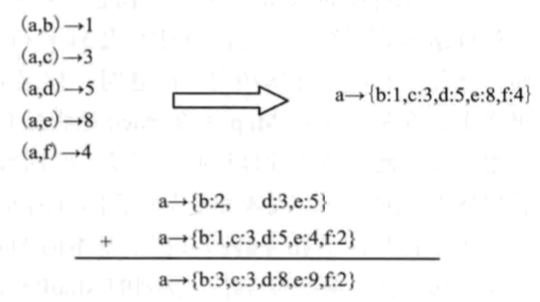
\includegraphics[width=4in]{figures/combine.png}
	\end{center}
\end{figure}
采用这种方法,会减少大量的中间结果键值对。
\subsection{结果对比}
以下表格是分别采用上述三种方法运行单词共现任务的耗时:
\begin{table}[htbp]
	\begin{center}
		\begin{tabular}{|c|c|}
			\hline
			\textbf{方法} & \textbf{单词共现任务耗时} \\ \hline
			baseline    & 66s               \\ \hline
			自定义键值对      & 56s               \\ \hline
			合并键值对       & 45s               \\ \hline
		\end{tabular}
	\end{center}
\end{table}\\
\indent 可看出,我们的优化是确实有效的,另外,采用将小键值对合并成大键值对的优化方法效果要好于自定义数据类型的方法。
\section{运行效果}
\subsection{集群运行}
\subsection{PageRank词云}
根据PageRank的结果,按照人物的PR值大小生成词云,可以直观的看出哪些人物是主角。
		\begin{figure}[ht]
			\centering
			
\includegraphics[scale=0.38]{figures/wordcloud.jpg}
			\caption{根据PageRank值生成词云}
		\end{figure}
\subsection{标签传播聚类}
根据PageRank和标签传播的结果,对人物关系图进行染色,可以看出哪些人物之间的关系密切,哪些人物属于同一本书。
\begin{figure}[ht]
	\centering
	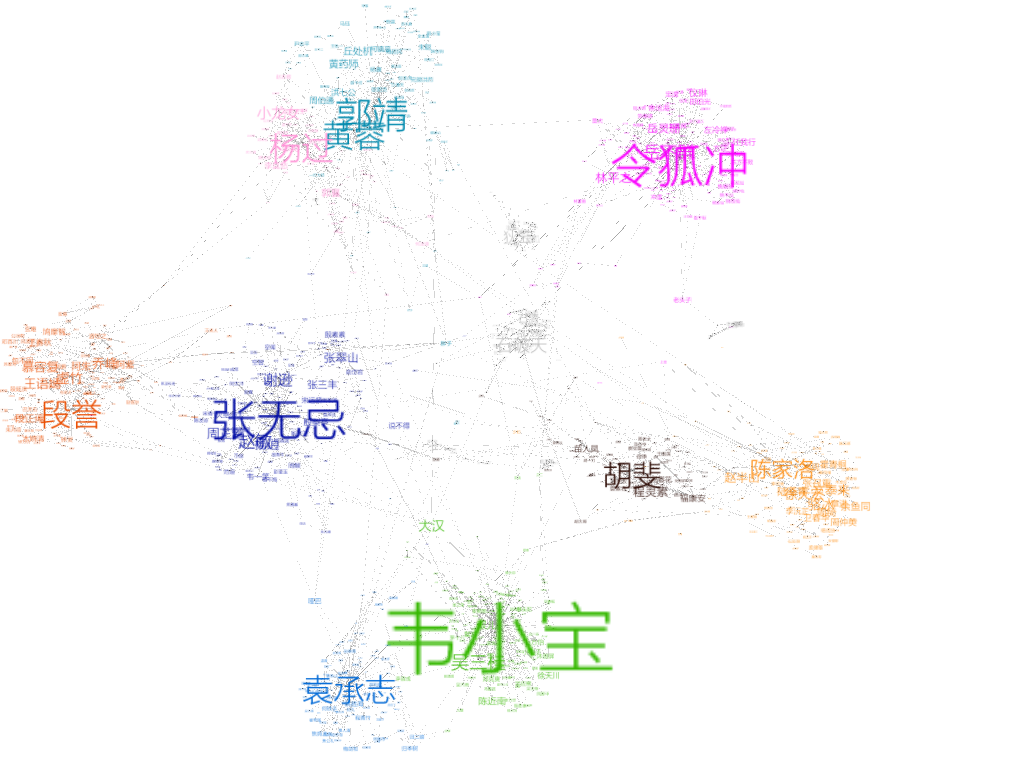
\includegraphics[scale=0.45]{figures/label_prop.png}
	\caption{标签传播结果可视化}
\end{figure}

\end{document}